%% ---------------------------------------------------------------------
%% Copyright 2014, Thales, IGN, Rémi Cura
%% 
%% This file contains the introduction of article
%% ---------------------------------------------------------------------


\todoall{utiliser point-set à la place de point cloud}

\section{Introduction}

\begin{figure*}[t!]
	\begin{center}
		\fbox{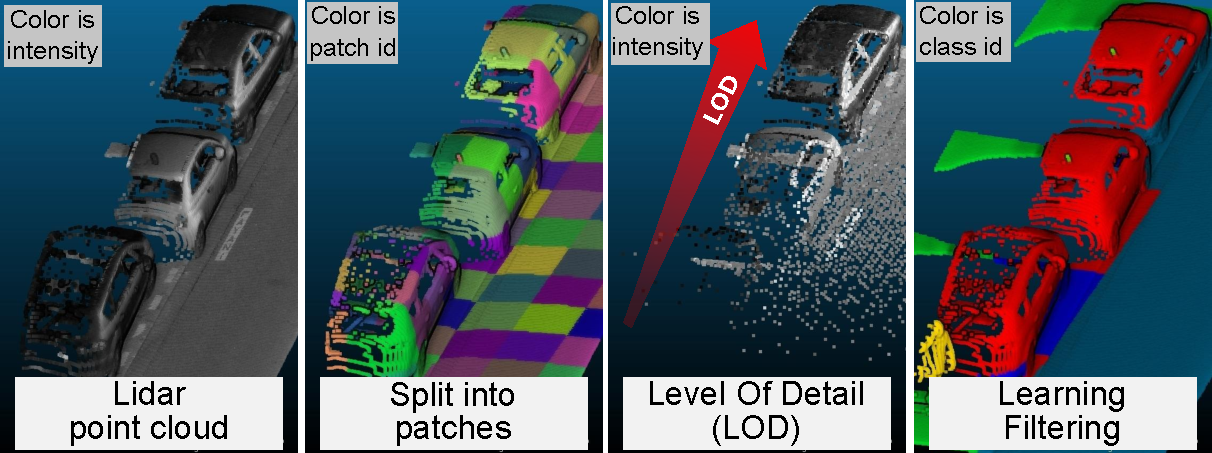
\includegraphics[width=\textwidth,keepaspectratio ]{./illustrations/chap2/lod_banner/banner_for_paper}}
		\caption{Graphical Abstract : a Lidar point cloud (1), is split it into patches (2) 
		and stored in the PCS (\cite{Cura2015}), patches are re-ordered to obtain free LOD 
		(3) (a gradient of LOD here), lastly the ordering by-product is a multiscale dimensionality descriptor used as a feature for learning and efficient filtering (4).} 
		\label{lod.fig:banner_image}
	\end{center}
\end{figure*} 

\subsection{Problem}   
	Democratisation of sensing device have resulted into an expansion of acquired point clouds.
	In the same time, acquisition frequency and precision of the Lidar device are also increasing,
	resulting in an explosion of number of points.
	
	Point cloud data usage is more common and no more limited to a specialized community.
	Datasets are now commonly in the multi billion point range and can not fit in computer memory.
	Furthermore, having the complete and fully detailed point cloud is impracticable, unnecessary, or even damageable for most applications.
	\todoall{
		point - prob de stockage car les tailles sont grandes,  -> problem d'utilisation . De plus les usages changes, se sont ouverts, donc il faut un accès facile
		Accès (simple pour les noob) , processing, stockage ->Big Data issue.
		} 
 
	\myimage{"./illustrations/chap2/two_reduction_strategy/two_reduction_strategy"}{Two strategies to limit the amount of points to work on.}{lod.fig:two_reduction} 
	\todoall{illustration : generalize , mettre un truc qui va avec filtering. , mettre un s et pas un z . 
		separation en noir fine plutot que gris}
	The ability to reduce the number of points is a key point for practical point cloud management and usage.
	There are basically two approaches to reduce the amount of data considered (See Figure \ref{lod.fig:two_reduction}) :
	by a \textbf{filtering} strategy based on data characteristics (position, time, semantic, etc.) which keeps only a portion the original data and/or a 
	\textbf{generalisation} of the data by replacing many points with fewer objects that represent appropriately those points. 
	For instance, in order to visualize massive point cloud, it's important to fetch only the appropriate points by selecting the ones which are visible (filtering) and which are the most representative of the scene (generalisation) at the same time.
	
	Many methods re compatible with filterign and/or generalisation.
	\todoall{many ùmethods perform filtering (petite liste, 3 papiers). Some other perform generalisation (petite liste).
		Cura2015 filtering et intorduit la generalisation avec des objets abstraits, mais n'utilise pasd de generalisation avec des points}
%	The Point Cloud Server (PCS) introduced by \cite{Cura2015} is compatible with both filtering and generalisation.
%	It covers the filtering part, with many possibilities (spatial, semantic, attributes, using vector and raster data, using metadata).
%	Nevertheless it uses a generalisation approach based only abstract types (bounding box, planes, stats, etc.), which limits its use to methods that are adapted to those types.
%	
%	Yet generalisation can be done generalised objects can be more abstract (geometric primitives like plane for example), or of the same type, i.e. simply some well chosen points (subset).
	Nevertheless it does not covers generalisation of points by points.
	
	\todoall{ paragrpahe suivant doit etre reecrit pour bien s'integrer}
	Robustness to variation of density is necessary because the sensing may be structured for the sensing device (for instance a Lidar may sense point using a constant angle), but not necessary for the sensed object (see Fig. \ref{lod.fig:irregular_sampling}). Furthermore,fusing multiple point clouds also produce non regular density.
	\myimage{"./illustrations/chap2/problem_in_sampling/regular_vs_irregular_sampling"}{Regular sensing does not imply regular sampling.}{lod.fig:irregular_sampling}.
	
	
	In this work we propose to extend the PCS to explore the generalisation of groups of points by choosing a representative subset of points (See Fig. \ref{lod.fig:two_reduction}).
	TODO
	We reduce successively the number of points by defining level which preserves the geometric characteristics of the underlying sensed object.
	Our method is designed to be efficient, robust to point density variation and can be used for many large point clouds processing, including visualisation.
	
\subsection{Related Work} 

	\todoall{
		generalisation : etudier dans les GIS
		
		ne pas melanger 2D et 3D 
		dire que la generalisation de point n a ete faite serieusement que en 2D, pas torp en 3D.
		Donc ocmmencer par la 2D.
		
		dire que la solution la plus puissante )(ui vient des GIS) est bonne n est pas transposable.
		Donc on cherche autre chose
		}
		
	This type of problem has been extensively studied in Geographical Information System (GIS)and other research field.
	It could be seen as compression, clustering, dimensionality reduction, or Level Of Detail (LOD) for visualisation.
	Sophisticated methods have been proposed to generalise 2D points for cartographic applications (\cite{Sester2001}, \cite{Schwartges2013}).
	\todoall{neanmoint : notre probleme données 3D lidar, et leur mehtods êuvent pas etre reutiliséées
		reparler de densité
		parler de complexité des methods (trop longs a calculer)}
	In both case, the goal is a very specific type of visualisation (cartography), and it obviously relies on having a 2D plan on which perform the methods.
	Applying directly such methods to point clouds would thus require to have access to surfaces of sensed objects.
	Yet, getting this surface (reconstruction) is a very hard challenge, sometime not even possible, and thus we can not rely on it.
	\todoall{conclusion : on peut pas utiliser leur truc}
	
	
	\todoall{reecrire en parlant a chaque fois des problemes et des oslutions apportées par les autres }
	Because the goal is to produce hierarchical levels of points, it seems natural to use a hierarchical structure to compute those levels.
	\cite{Rusinkiewicz2000} use a Bounding Sphere Hierarchy for a visualisation application.
	On the other hand, Octree (\cite{Meagher1982}) have become the de-facto choice.
	Indeed, they can be build efficiently ordering points by Morton (or GeoHash \cite{Sabo2014}) order (\cite{Feng2014}).
	\todoall{mettre une citation sur morton}
	Octree can even be created out of memory for extremely large point clouds (\cite{Baert2014}). 
	\todoall{mettre sous forme d avantage de l octree}
	Moreover, their regularity allows efficient representation and compression (\cite{Schnabel2006,Huang2006}), as well as fast geospatial access to data (\cite{Elseberg2013}).
	\todoall{parler du fait qu'en general les octree sont utiliser que de l indexation}
	Octree are also natural condidates to nesting (i.e. create a hierarchy of octrees with various resolution and occupancy, as in \cite{Hornung2013}). 
	\todoall{conclusion sur les octree : probleme des octree : stockage en exterieur, compatibilité, etc.
		toutes les methodes prennent le centroide
		}
	
	
	\todoall[]{neanmoins, en 3D, choix ps vraiment justifier alors que c'est important, mais en 2D, choix etudier par .. preiciser que quadtree est un octree dimension 2.
		Preciser qu'on utiliser les conclusions de la 2D pour la 3D, car l etude n existe pas en 3D}
	\cite{Bereuter2015} recently gave an overview of how quad tree can be used for point generalisation.
	The steps are first to compute a tree for the point cloud.
	Then, the point generalisation at a given level is obtained for each cell of the same tree level, by having one point represent all the points of this cell.
	
	There are two methods to choose a point representing the others. The first one is to select on points among all ('select').
	The second method is to create a new point that will represent well the others ('aggregate'). 
	Both these methods can use geometry of points, but also other attributes.
	
	In theory, choosing an optimal point would also depend on application.
	For instance lets consider a point cloud containing a classification, and suppose the application is to visually identify the presence of a very rarely present class C.
	In this case a purely geometrical LOD would probably hide C until the very detailed levels. On the opposite, prefering a point classified in C whenever possible would be optimal for this application.
	
	However, a LOD method has to be agnostic regarding point clouds,
	and point clouds may have many attributes of various type and meaning, as long as many applications.
	Therefore, most methods use only the minimal common factor of possible attributes, that is spatial coordinates. 
	For visualisation applications, aggregating points seems to be the most popular choice \cite{Schutz2015,Hornung2013,Elseberg2013}. with aggregating functions like centroids of the points or centroid of the cell.
	
	All of this methods also use an aggregative function (barycentre of the points, centroid of the cell) to represent the points of a cell.
	Using the barycentre seems intuitive, as it is also the point that minimize the squared distance to other points in the cell, and thus a measure of geometric error.
	
	However, using the 'aggregate' rather than 'select' strategy necessary introduces aggregating errors
	 (as opposed to potential aliasing error), and is less agnostic.
	Indeed, aggregating means fabricating new points, and also necessitate a way to aggregate for each attributes, which might be complex (for instance semantic aggregating; a point of trash can and a point of bollard could be aggregated into a point of street furniture).
	This might not be a problem for visualization application.
	Yet our goal is to provide LOD for other processing methods, which might be influenced by aggregating errors.
	Furthermore, the barycentre is very sensible to density variations.
	
	Therefore, we prefer to use a 'select' strategy. The point to be selected is the closest to the centroid of the octree cell.
	If the point cloud density is sufficient this strategy produces a nearly regularly sampled point cloud, which might be a statistical advantage for processing methods. 
	To establish a parallel with statistics, picking one point per cell is akin to a Latin Hypercube (see \cite{McKay1979}).
	Avoiding the averaging strategy might also increase the quantity of information than can be retrieved (similar to compressed sensing, see \cite{Fornasier2010}).
	
	
	We note that most of the LOD systems seems to have been created to first provide a fast access to point (spatial indexing), and then adapted to provide LOD.
	Using the PCS, we can separate the indexing part, and the LOD scheme. From this stems less design constraints, more possibilities, and a method than is not dedicated to only one application (like visualisation). 
	

\subsection{Contribution}

	This work re-uses and combines existing and well established methods with a focus on simplicity and efficiency. As such, all the methods are tested on billions scale point cloud, and are Open Source for sake of reproducibility test and improvements
	
	\todoall{mettre une liste latex item} 
	
	Our first contribution (Section \ref{lod.method.order}) is to store the LOD implicitly in the ordering of the points rather than externally, avoiding any data duplication.
	Thus, we don't duplicate information, and the more we read points, the more precise of an approximation of the point cloud we get. If we read all the points, we have the original point cloud.
	
	The second contribution (MidOc, Section \ref{lod.method:midoc}) is a simple way to order points in order to have an increasingly better geometric approximation of the point cloud when following this order.
	
	The third contribution (Section \ref{lod.method.dimdescriptor}) is to show that this ordering embed information about the dimensionality of the sensed object,
	to the point of being a simple multi-scale dimensionality descriptor.
	We demonstrate the interest of this descriptor by comparing it to a state of the art dimensionality descriptor, then by assessing it potential by performing a Random Forest classification that can then be used for very fast pre-filtering of points, and other applications.
		
	
%\subsection{Plan of the article}
	Section~\ref{lod.sec:method} presents the LOD solution, how it produces a dimensionality descriptor, and how this can leveraged for classification.  
	Section~\ref{lod.sec:result} reports on the experiments validating the methods.
	Finally, the details, the limitations, and potential applications are discussed in Section~\ref{lod.sec:discussion}.
	
